\documentclass[11pt, a4paper]{article}

\usepackage[utf8]{inputenc}
\usepackage[T1]{fontenc}
\usepackage{geometry}
\geometry{a4paper, margin=1in}
\usepackage{amsmath, amssymb, amsthm}
\usepackage{graphicx}
\usepackage{listings}
\usepackage{xcolor}
\usepackage{hyperref}
\usepackage{enumitem}
\usepackage{float} % For [H] option in figures/tables
\usepackage{caption}
\usepackage{booktabs} % For better table lines
\usepackage{tikz}
\usetikzlibrary{shapes, arrows, positioning, shadows, patterns}
\usepackage{tikz-uml} % For UML diagrams

% Listings configuration for C++
\definecolor{codegreen}{rgb}{0,0.6,0}
\definecolor{codegray}{rgb}{0.5,0.5,0.5}
\definecolor{codepurple}{rgb}{0.58,0,0.82}
\definecolor{backcolour}{rgb}{0.95,0.95,0.92}

\lstdefinestyle{cppstyle}{
    backgroundcolor=\color{backcolour},   
    commentstyle=\color{codegreen},
    keywordstyle=\color{magenta},
    numberstyle=\tiny\color{codegray},
    stringstyle=\color{codepurple},
    basicstyle=\ttfamily\footnotesize,
    breakatwhitespace=false,         
    breaklines=true,                 
    captionpos=b,                    
    keepspaces=true,                 
    numbers=left,                    
    numbersep=5pt,                  
    showspaces=false,                
    showstringspaces=false,
    showtabs=false,                  
    tabsize=2,
    language=C++
}
\lstset{style=cppstyle}

\hypersetup{
    colorlinks=true,
    linkcolor=blue,
    filecolor=magenta,      
    urlcolor=cyan,
    pdftitle={Rubik's Cube Solver Project Report},
    pdfpagemode=FullScreen,
}

\title{Rubik's Cube Solver: Project Documentation}
\author{Your Name} % Replace with your name
\date{\today}

\begin{document}

\maketitle
\thispagestyle{empty}
\newpage

\tableofcontents
\thispagestyle{empty}
\newpage
\setcounter{page}{1}

\section{Introduction}
This document details the design, architecture, and implementation of a C++ application, "RubiksCubeSolver". The primary goal of this project is to provide a visual representation of a Rubik's Cube and implement an autonomous solver using Thistlethwaite's algorithm. The application utilizes SDL2 for graphics and user interaction, and C++20 features for efficient cube state manipulation. This report covers the overall architecture, cube representation, solving algorithms, database utilization, and the general data flow within the system.

\section{Overall Architecture and Flow}
The RubiksCubeSolver project is structured into several key modules that interact to deliver its functionality: the \texttt{Engine} for graphics and control, the \texttt{Cube} for state representation, the \texttt{Solver} for algorithmic solutions, and \texttt{Util} for auxiliary functions.

\subsection{System Startup and Control Flow}
Execution begins with \texttt{main.cpp}, which instantiates an \texttt{Engine} object and invokes its \texttt{run()} method. The \texttt{Engine} then initializes SDL2, creates the main window, and enters a main loop. Within this loop, it processes user input, updates the cube's state (either through user moves or solver actions), and renders the cube on the screen.

\begin{enumerate}
    \item \textbf{\texttt{main.cpp}}: Entry point. Creates and runs the \texttt{Engine}.
    \item \textbf{\texttt{Engine}}: Manages the application lifecycle, SDL2 window, rendering, event polling, and interaction with the \texttt{Cube} and \texttt{Solver}.
    \item \textbf{\texttt{Cube}}: Represents the Rubik's Cube state and provides methods for manipulation (rotations, getting colors, etc.).
    \item \textbf{\texttt{Solver} (Thistlethwaite)}: Implements the solving algorithm. It uses \texttt{Searcher} (A* or IDDFS), \texttt{Database}s, and \texttt{Goal} definitions.
    \item \textbf{\texttt{Util}}: Contains helper classes like \texttt{DatabaseGenerator}, \texttt{Indexer}, and \texttt{SearchUtil}.
\end{enumerate}

\subsection{UML Class Diagram}
A simplified UML class diagram illustrating the main components and their relationships is shown in Figure \ref{fig:uml_diagram}.

\begin{figure}[H]
    \centering
    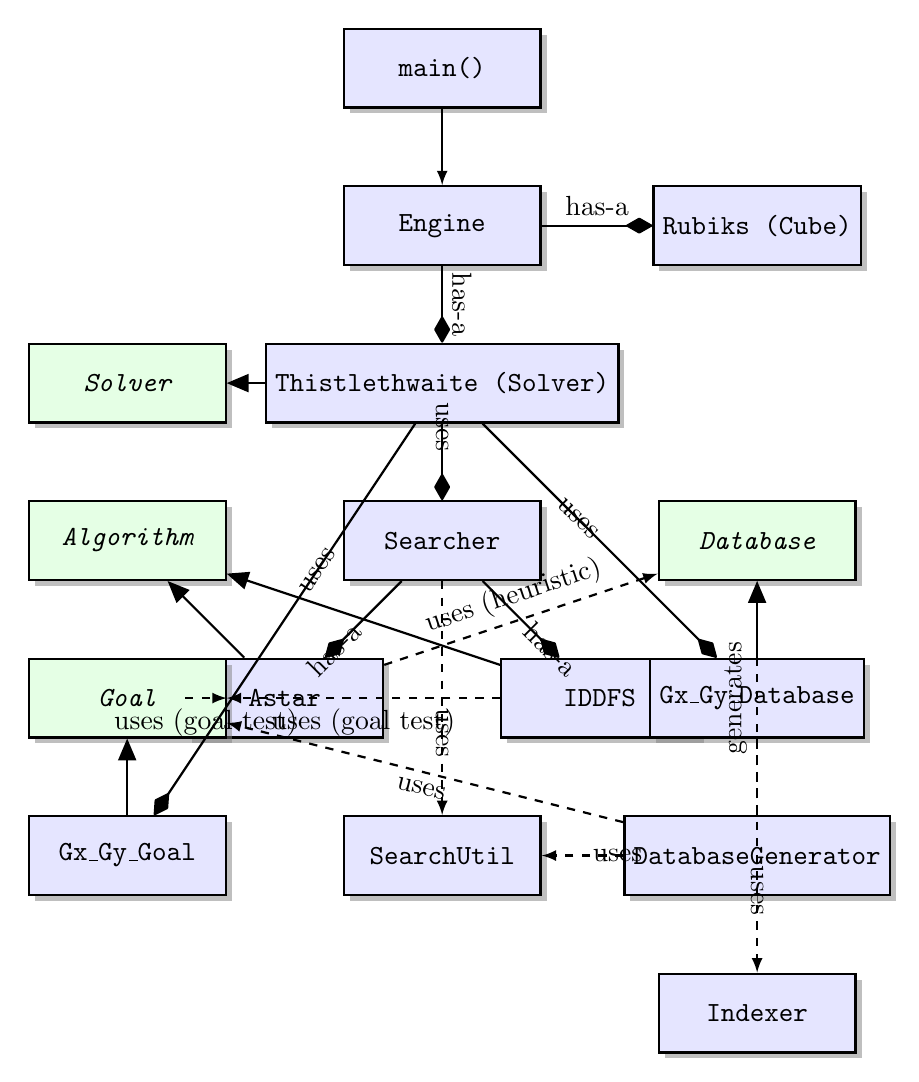
\begin{tikzpicture}[
        % Define styles for UML elements
        class/.style={rectangle, draw=black, fill=blue!10, thick, minimum height=1cm, minimum width=2.5cm, text centered, drop shadow},
        interface/.style={rectangle, draw=black, fill=green!10, thick, minimum height=1cm, minimum width=2.5cm, text centered, drop shadow, font=\itshape},
        aggregation/.style={-diamond, thick},
        composition/.style={-latex, fill=black, thick}, % Filled diamond for composition
        inheritance/.style={-triangle 45, thick},
        association/.style={-latex, thick},
        dashed_association/.style={-latex, thick, dashed}
    ]

    % Nodes
    \node[class] (Main) at (0,10) {\texttt{main()}};
    \node[class] (Engine) at (0,8) {\texttt{Engine}};
    \node[class] (Rubiks) at (4,8) {\texttt{Rubiks (Cube)}};
    \node[class] (Thistlethwaite) at (0,6) {\texttt{Thistlethwaite (Solver)}};
    \node[interface] (SolverInterface) at (-4,6) {\texttt{Solver}}; % Abstract Solver
    \node[class] (Searcher) at (0,4) {\texttt{Searcher}};
    \node[interface] (Algorithm) at (-4,4) {\texttt{Algorithm}}; % Abstract Algorithm
    \node[class] (Astar) at (-2,2) {\texttt{Astar}};
    \node[class] (IDDFS) at (2,2) {\texttt{IDDFS}};
    \node[interface] (Database) at (4,4) {\texttt{Database}}; % Abstract Database
    \node[class] (SpecificDB) at (4,2) {\texttt{Gx\_Gy\_Database}};
    \node[interface] (Goal) at (-4,2) {\texttt{Goal}}; % Abstract Goal
    \node[class] (SpecificGoal) at (-4,0) {\texttt{Gx\_Gy\_Goal}};
    \node[class] (DatabaseGenerator) at (4,0) {\texttt{DatabaseGenerator}};
    \node[class] (Indexer) at (4,-2) {\texttt{Indexer}};
    \node[class] (SearchUtil) at (0,0) {\texttt{SearchUtil}};

    % Relationships
    \draw[association] (Main) -- (Engine);
    \draw[aggregation] (Engine) -- (Rubiks) node[midway, above, sloped] {has-a};
    \draw[aggregation] (Engine) -- (Thistlethwaite) node[midway, above, sloped] {has-a};
    
    \draw[inheritance] (Thistlethwaite) -- (SolverInterface);
    \draw[aggregation] (Thistlethwaite) -- (Searcher) node[midway, left, sloped] {uses};
    \draw[aggregation] (Thistlethwaite) -- (SpecificDB) node[midway, right, sloped, pos=0.3] {uses};
    \draw[aggregation] (Thistlethwaite) -- (SpecificGoal) node[midway, left, sloped, pos=0.3] {uses};

    \draw[aggregation] (Searcher) -- (Astar) node[midway, left, sloped] {has-a};
    \draw[aggregation] (Searcher) -- (IDDFS) node[midway, right, sloped] {has-a};
    \draw[inheritance] (Astar) -- (Algorithm);
    \draw[inheritance] (IDDFS) -- (Algorithm);
    
    \draw[dashed_association] (Astar) -- (Database) node[midway, above, sloped] {uses (heuristic)};
    \draw[dashed_association] (Astar) -- (Goal) node[midway, below, sloped] {uses (goal test)};
    \draw[dashed_association] (IDDFS) -- (Goal) node[midway, below, sloped] {uses (goal test)};
    
    \draw[inheritance] (SpecificDB) -- (Database);
    \draw[inheritance] (SpecificGoal) -- (Goal);
    
    \draw[dashed_association] (DatabaseGenerator) -- (Database) node[midway, above, sloped] {generates};
    \draw[dashed_association] (DatabaseGenerator) -- (Goal) node[midway, below, sloped] {uses};
    \draw[dashed_association] (SpecificDB) -- (Indexer) node[midway, right, sloped] {uses};
    \draw[dashed_association] (Searcher) -- (SearchUtil) node[midway, right, sloped] {uses};
    \draw[dashed_association] (DatabaseGenerator) -- (SearchUtil) node[midway, right, sloped] {uses};

    \end{tikzpicture}
    \caption{Simplified UML Class Diagram of the Rubik's Cube Solver.}
    \label{fig:uml_diagram}
\end{figure}

\section{Cube Representation and Manipulation (\texttt{Cube} Module)}
The core of the Rubik's Cube logic resides in the \texttt{Rubiks} class, defined in \texttt{Cube.h} and implemented in \texttt{Cube.cpp}.

\subsection{Data Structures and In-Memory Representation}
\begin{itemize}
    \item \textbf{Internal State (\texttt{m\_cube})}: The cube's state is primarily stored in \texttt{std::array<ECOLOUR, 48> m\_cube;}. Each element represents the color of one of the 48 non-center facelets. Center pieces are considered fixed.
    \item \textbf{Enums for Clarity}:
    \begin{itemize}
        \item \texttt{EFACE}: Defines the six faces (U, L, F, R, B, D).
        \item \texttt{ECOLOUR}: Defines the six colors (W, O, G, R, B, Y).
        \item \texttt{EPIECE}: Symbolic names for the 20 cubies (12 edges, 8 corners).
        \item \texttt{EEDGE}, \texttt{ECORNER}: Symbolic names for individual facelets of edges and corners, mapping to indices in \texttt{m\_cube}.
        \item \texttt{EMOVE}: Defines all possible moves (clockwise, counter-clockwise, 180-degree).
    \end{itemize}
    \item \textbf{Face Representation for Rotation}: For efficient rotations, each face (8 stickers) can be treated as a \texttt{uint64\_t} (8 bytes, 1 byte per color sticker). Methods \texttt{getFace()} and \texttt{setFace()} handle this conversion using \texttt{memcpy}. C++20's \texttt{std::rotl} and \texttt{std::rotr} are used on this \texttt{uint64\_t} for fast bitwise rotation of facelets.
\end{itemize}

\subsection{Key Methods of the \texttt{Rubiks} Class}
\begin{description}
    \item[\texttt{Rubiks()}] Constructor, initializes the cube to a solved state via \texttt{resetCube()}.
    \item[\texttt{resetCube()}] Sets all facelets to their solved state colors.
    \item[\texttt{isSolved() const}] Checks if the cube is in the solved configuration by comparing each face's \texttt{uint64\_t} representation to the solved state.
    \item[\texttt{rotateFaceCW(EFACE face)}, \texttt{rotateFaceCCW(EFACE face)}, \texttt{rotateFace180(EFACE face)}] These methods rotate the stickers on the specified face. They use \texttt{std::rotl} or \texttt{std::rotr} on the \texttt{uint64\_t} face representation.
    \item[\texttt{rotateAdjacents(const adjacentIndices\_t\& adj)}, \texttt{rotateAdjacents180(const adjacentIndices\_t\& adj)}] These methods update the 8 facelets on adjacent faces that are affected by a face turn. The \texttt{adjacentIndices\_t} (an array of 8 indices) specifies which facelets to move.
    \item[\texttt{performMove(EMOVE move)}] A high-level function that takes an \texttt{EMOVE} enum and calls the appropriate low-level rotation methods (e.g., \texttt{U()}, \texttt{Lp()}).
    \item[\texttt{U(), Up(), U2(), L(), ... D2()}] Specific methods for each possible move. They combine calls to \texttt{rotateFace...} and \texttt{rotateAdjacents...} with hardcoded indices for the adjacent facelets.
    \item[\texttt{getColour(uint8\_t index/ECORNER index/EEDGE index) const}] Retrieves the color of a specific facelet.
    \item[\texttt{getPieceInd(EPIECE piece) const}] Returns a unique index for a piece (edge or corner) based on its current colors and location. This is crucial for database lookups.
    \item[\texttt{getEdgeOrientation(const edge\_t\& edge) const}, \texttt{getCornerOrientation(const corner\_t\& corner) const}] Determine the orientation (flip or twist) of an edge or corner piece. Essential for defining goal states in Thistlethwaite's algorithm.
\end{description}
The use of \texttt{uint64\_t} for face representation and C++20's bitwise rotation functions (\texttt{std::rotl}, \texttt{std::rotr}) significantly optimizes the speed of face sticker manipulation.

\section{The Solving Engine (\texttt{Solver} Module)}
The project employs Thistlethwaite's algorithm to solve the Rubik's Cube. This algorithm breaks the problem into a sequence of four sub-problems, each with a more restricted set of allowed moves.

\subsection{Thistlethwaite's Algorithm}
The \texttt{Thistlethwaite} class manages the overall solving process. It iterates through four groups (G0 $\rightarrow$ G1, G1 $\rightarrow$ G2, G2 $\rightarrow$ G3, G3 $\rightarrow$ G4), each aiming to achieve a specific intermediate state.
\begin{itemize}
    \item \textbf{G0 $\rightarrow$ G1}:
        \begin{itemize}
            \item \textbf{Goal}: Orient all 12 edges correctly. "Good" orientation means an edge can be solved without 90-degree U/D face turns later.
            \item \textbf{Allowed Moves}: All moves.
            \item \textbf{Database}: \texttt{G0\_G1\_Database} (2048 states for edge orientations).
            \item \textbf{Goal Check}: \texttt{G0\_G1\_Goal::contented()}.
        \end{itemize}
    \item \textbf{G1 $\rightarrow$ G2}:
        \begin{itemize}
            \item \textbf{Goal}: Orient all 8 corners correctly and place the 4 M-slice (middle layer) edges into the M-slice.
            \item \textbf{Allowed Moves}: U/D 90-degree turns are disallowed (only U2, D2, and all L, R, F, B moves).
            \item \textbf{Database}: \texttt{G1\_G2\_Database} (1,082,565 states for corner orientations and M-slice edge positions).
            \item \textbf{Goal Check}: \texttt{G1\_G2\_Goal::contented()}.
        \end{itemize}
    \item \textbf{G2 $\rightarrow$ G3}:
        \begin{itemize}
            \item \textbf{Goal}: Place all edges into their correct slices (E, S, M) and corners into their correct orbits (tetrads), such that the cube is solvable with only 180-degree turns. Parity is also corrected.
            \item \textbf{Allowed Moves}: U/D/F/B 90-degree turns are disallowed (only L, R 90-degree turns and all 180-degree turns).
            \item \textbf{Database}: \texttt{G2\_G3\_Database} (29,400 states for edge slice positions, corner orbits, and parity).
            \item \textbf{Goal Check}: \texttt{G2\_G3\_Goal::contented()}.
        \end{itemize}
    \item \textbf{G3 $\rightarrow$ G4 (Solved)}:
        \begin{itemize}
            \item \textbf{Goal}: Solve the cube completely.
            \item \textbf{Allowed Moves}: Only 180-degree turns (U2, D2, L2, R2, F2, B2).
            \item \textbf{Database}: \texttt{G3\_G4\_Database} (663,552 states for permutations of pieces within their orbits).
            \item \textbf{Goal Check}: \texttt{G3\_G4\_Goal::contented()} (calls \texttt{Rubiks::isSolved()}).
        \end{itemize}
\end{itemize}
For each phase, a search algorithm finds the shortest sequence of allowed moves to reach the next phase's goal state.

\subsection{Search Algorithms (\texttt{Searcher})}
The \texttt{Searcher} class encapsulates the search algorithms used by the solver.
\begin{description}
    \item[A* Algorithm (\texttt{Astar})]:
    A heuristic search algorithm that aims to find the shortest path to a goal.
    \begin{itemize}
        \item It uses a priority queue to explore nodes with the lowest $f(n) = g(n) + h(n)$ value, where:
            \begin{itemize}
                \item $g(n)$ is the actual cost (number of moves) from the start state to node $n$.
                \item $h(n)$ is the heuristic estimate of the cost from node $n$ to the goal. In this project, $h(n)$ is retrieved from the pre-calculated pattern \texttt{Database} for the current phase. The database stores the minimum number of moves required to reach the phase's goal state from any given configuration relevant to that phase.
            \end{itemize}
        \item If \texttt{database[currentState] == 0}, it means the current state is a goal state for that phase according to the database. The \texttt{Goal::contented()} method then provides the final verification.
        \item The A* search significantly speeds up finding solutions for each phase by intelligently guiding the search towards promising states.
    \end{itemize}
    \item[Iterative Deepening Depth-First Search (IDDFS) (\texttt{IDDFS})]:
    A brute-force search algorithm that combines the benefits of DFS (low memory usage) and BFS (finds shortest path).
    \begin{itemize}
        \item It performs a series of depth-limited DFS searches, incrementing the depth limit with each iteration (depth = 0, 1, 2, ...).
        \item It does not require a heuristic database but is generally slower than A* for these problems. It can serve as a fallback or for phases where database generation is impractical or for comparison.
        \item The current implementation seems to use A* primarily when a database is available for a group, and IDDFS might be an alternative or for groups without a database (though all Thistlethwaite groups here have databases).
    \end{itemize}
\end{description}

\subsection{Pattern Databases (\texttt{Database})}
Pattern databases are crucial for the efficiency of the Thistlethwaite solver, particularly when using A*.
\begin{itemize}
    \item \textbf{Purpose}: They store the minimum number of moves required to reach the goal state of a specific phase from any relevant abstract state of that phase. This value serves as an admissible and consistent heuristic for the A* search algorithm.
    \item \textbf{Generation (\texttt{DatabaseGenerator})}:
        \begin{itemize}
            \item Databases are pre-calculated by the \texttt{DatabaseGenerator} class.
            \item It performs a breadth-first search (implemented as iterative deepening in \texttt{databaseSearcher}) starting from the goal state(s) of a phase, working backward.
            \item For each reachable state, it records its depth (distance from the goal) in the database file.
            \item The \texttt{Goal} object for the phase defines the allowed moves for this backward search.
            \item Files are stored in the \texttt{./Data/Thistlethwaite/} directory (e.g., \texttt{G0}, \texttt{G1}).
        \end{itemize}
    \item \textbf{Structure and Usage}:
        \begin{itemize}
            \item The base \texttt{Database} class handles loading from/writing to files and provides an interface for accessing depth values.
            \item Derived classes (e.g., \texttt{G0\_G1\_Database}, \texttt{G1\_G2\_Database}) implement a virtual method \texttt{getInd(const Rubiks\& cube) const}. This method maps the current state of the \texttt{Rubiks} cube to a unique integer index. This indexing is complex and specific to the characteristics of each phase (e.g., edge orientations for G0, corner orientations and M-slice edge positions for G1). It often involves combinatorial calculations using the \texttt{Indexer} utility.
            \item During A* search, \texttt{database[cubeState]} (which internally calls \texttt{getInd}) retrieves the heuristic value.
        \end{itemize}
    \item \textbf{Optimization}: By providing an accurate lower bound on the number of moves to the goal, pattern databases drastically prune the search space explored by A*, leading to very fast solution times for each phase. Without them, solving would be computationally infeasible for the later, more complex phases.
\end{itemize}

\section{Graphics and User Interaction (\texttt{Engine} Module)}
The \texttt{Engine} class is responsible for all visual aspects and user input handling using the SDL2 library.

\begin{itemize}
    \item \textbf{SDL2 Initialization (\texttt{Engine::init()})}: Initializes SDL, creates the main window (\texttt{SDL\_Window}) and renderer (\texttt{SDL\_Renderer}). It also sets up color palettes and initial positions/sizes for the facelet rectangles.
    \item \textbf{Main Loop (\texttt{Engine::mainLoop()})}: The heart of the engine, running continuously until the user quits. In each iteration, it:
        \begin{enumerate}
            \item Calls \texttt{Engine::pollEvents()} to process user input.
            \item Calls \texttt{Engine::update()} to handle time-based logic (like animated solving).
            \item Calls \texttt{Engine::render()} to draw the current state of the cube.
            \item Manages frame timing to achieve a target FPS.
        \end{enumerate}
    \item \textbf{Event Handling (\texttt{Engine::pollEvents()})}:
        \begin{itemize}
            \item Detects keyboard presses for cube manipulations (U, L, F, R, B, D, with Shift for prime, Ctrl for 2-moves). These directly call methods on the \texttt{m\_cube} object (e.g., \texttt{m\_cube.U()}).
            \item Handles commands like scramble (\texttt{SDLK\_s} $\rightarrow$ \texttt{Engine::scramble()}), reset (\texttt{SDLK\_ESCAPE} $\rightarrow$ \texttt{m\_cube.resetCube()}), and solve (\texttt{SDLK\_F1}).
            \item When F1 is pressed, it calls \texttt{m\_thistlethwaite.solve(m\_cube)}. The returned solution (a vector of moves) is then stored.
        \end{itemize}
    \item \textbf{Rendering (\texttt{Engine::render()})}:
        \begin{itemize}
            \item Clears the screen.
            \item Iterates through the 6 center facelets and 48 other facelets.
            \item For each non-center facelet, it gets its current color from \texttt{m\_cube.getColour(sticker\_index)}.
            \item Uses \texttt{SDL\_SetRenderDrawColor} and \texttt{SDL\_RenderFillRect} to draw the colored rectangle for each facelet at its pre-calculated screen position.
        \end{itemize}
    \item \textbf{Animated Solving}: When a solution is generated, the \texttt{Engine::update()} method applies one move from the solution sequence at a time, with a fixed delay (\texttt{ANIMATED\_MOVE\_DELAY}) between moves, allowing the user to visually follow the solution steps.
\end{itemize}

\section{Utility Modules (\texttt{Util} Module)}
The \texttt{Util} directory contains several helper classes:
\begin{itemize}
    \item \textbf{\texttt{DatabaseGenerator}}: As described earlier, responsible for the offline pre-calculation of pattern databases. It uses a search strategy (iterative deepening BFS-like) starting from goal states defined by a \texttt{Goal} object.
    \item \textbf{\texttt{Indexer} (\texttt{indexer.h})}: Provides tools for combinatorial indexing, such as calculating unique indices for permutations and combinations. This is heavily used by the specific \texttt{Database} classes' \texttt{getInd()} methods to map complex cube states (like the arrangement of certain pieces) to a single integer index for database lookup.
    \item \textbf{\texttt{SearchUtil}}: Contains utility functions for search algorithms, most notably \texttt{isRedundant(currentMove, lastMove)}. This function helps prune search trees by avoiding obviously non-optimal move sequences (e.g., U followed immediately by U', or R R R).
    \item \textbf{\texttt{RandomNumGenerator}}: A simple utility for generating random numbers, used by \texttt{Engine::scramble()} to create random scramble sequences.
    \item \textbf{\texttt{Timer}}: A utility to measure execution time, used for benchmarking database generation and solving times.
\end{itemize}

\section{Data Flow Examples}
\subsection{User Performing a Manual Move}
\begin{enumerate}
    \item User presses a key (e.g., 'U').
    \item \texttt{Engine::pollEvents()} detects the SDL keydown event.
    \item \texttt{Engine} calls the corresponding method on its \texttt{m\_cube} instance (e.g., \texttt{m\_cube.U()}).
    \item The \texttt{Rubiks::U()} method modifies the internal \texttt{m\_cube} array by calling \texttt{rotateFaceCW(EFACE::U)} and \texttt{rotateAdjacents(...)}.
    \item On the next frame, \texttt{Engine::render()} reads the updated state from \texttt{m\_cube} via \texttt{m\_cube.getColour()} for each facelet and redraws the cube on the screen.
\end{enumerate}

\subsection{Scrambling the Cube}
\begin{enumerate}
    \item User presses 'S'.
    \item \texttt{Engine::pollEvents()} calls \texttt{Engine::scramble()}.
    \item \texttt{Engine::scramble()} uses \texttt{RandomNumGenerator} to pick a sequence of random moves. \texttt{SearchUtil::isRedundant()} may be used to ensure a more effective scramble.
    \item For each random move, \texttt{m\_cube.performMove()} is called, updating the cube's state.
    \item \texttt{Engine::render()} displays the progressively scrambled cube.
\end{enumerate}

\subsection{Initiating and Displaying a Solution}
\begin{enumerate}
    \item User presses 'F1'.
    \item \texttt{Engine::pollEvents()} calls \texttt{m\_thistlethwaite.solve(m\_cube)}.
    \item \texttt{Thistlethwaite::solve()} iterates through its four phases (G0-G1, G1-G2, G2-G3, G3-G4):
        \begin{enumerate}
            \item For each phase, it calls \texttt{m\_searcher.astar.search()} (or \texttt{iddfs.search()}) with the current cube state, the phase's specific \texttt{Goal} object, and its \texttt{Database} object.
            \item The search algorithm (e.g., A*) uses the \texttt{Database} for heuristics and the \texttt{Goal::contented()} method to check for phase completion.
            \item A sequence of moves for that phase is returned. These moves are applied to an internal copy of the cube state within the solver, and the moves are appended to the total solution list.
        \end{enumerate}
    \item \texttt{Thistlethwaite::solve()} returns the complete solution (a \texttt{std::vector<Rubiks::EMOVE>}) to the \texttt{Engine}.
    \item The \texttt{Engine} stores this solution in \texttt{m\_solutionMoves} and sets \texttt{m\_isSolvingAnimated = true}.
    \item In subsequent calls to \texttt{Engine::update()}, if \texttt{m\_isSolvingAnimated} is true and the delay has passed:
        \begin{enumerate}
            \item The next move from \texttt{m\_solutionMoves} is fetched.
            \item \texttt{m\_cube.performMove()} is called with this move.
            \item \texttt{m\_lastAnimatedMoveTime} is updated.
        \end{enumerate}
    \item \texttt{Engine::render()} continuously redraws the cube, showing the animated solution.
\end{enumerate}

\section{Conclusion}
The RubiksCubeSolver project successfully combines graphical representation with advanced algorithmic solving. The modular design allows for clear separation of concerns between cube logic, solving strategies, and user interface. The implementation of Thistlethwaite's algorithm, supported by A* search and pre-calculated pattern databases, enables efficient and rapid solving of the Rubik's Cube. The use of SDL2 provides an intuitive visual interface for users to interact with and observe the cube. This project serves as a comprehensive example of applying computer science principles to solve a classic combinatorial puzzle.

\end{document}